%Fiquemos com Deus e Nossa Senhora!
%Sao Jose de Cupertino rogai por nos!!
%Honra teu pai e tua mae!
% ### Uses XeLaTeX ### %
% ### Needs beamer-master ### %
\documentclass[aspectratio=169]{beamer} %. Aspect Ratio 16:9

\usetheme{AI2} % beamerthemeSprace.sty
\usepackage[portuguese]{babel}
\usepackage[utf8]{inputenc}
\usepackage[T1]{fontenc}
\usepackage{ragged2e,bm,oubraces,tikz}
\DeclareMathOperator*{\argmin}{arg\,min}
\DeclareMathOperator*{\argmax}{arg\,max}

\newcommand*\mycirc[1]{%
  \begin{tikzpicture}
    \node[draw,circle,inner sep=2pt] {#1};
  \end{tikzpicture}}
  
% DATA FOR FOOTER
\date{2025}
\title{- Análise de Algoritmos}
\author{João Paulo Papa}
\institute{Análise de Algoritmos}

\begin{document}
% ####################################
% FIRST SLIDE 						:: \SliTit{This is the Title of the Talk}{A. B. Name}{Sprace}
% SUB-TITLE SLIDE 					:: \SliSubTit{<title>}{<explanation}
% SUB-SUB-TITLE SLIDE				:: \SliSubSubTit{<title>}{<explanation}
% SLIDE WITH TITLE 					:: \SliT{Title}{Content}
% SLIDE NO TITLE 						:: \Sli{Content} 
% SLIDE DOUBLE COLUMN WITH TITLE 	:: \SliDT{Title}{First Column}{Second Column}
% SLIDE DOUBLE COLUMN NO TITLE 		:: \SliD{First Column}{Second Column}
% SLIDE ADVANCED WITH TITLE 			:: \SliAdvT{Title}{Content}
% SLIDE ADVANCED NO TITLE 			:: \SliAdv{Content}
% SLIDE ADVANCED DOUBLE WITH TITLE 	:: \SliAdvDT{Title}{First Column}{Second Column}
% SLIDE ADVANCED DOUBLE NO TITLE 	:: \SliAdvD{First Column}{Second Column}
% SLIDE BLACK						:: \Black{ <Content> }
% SLIDE WHITE						:: \White{ <Content> }
% ITEMIZATION 						:: \begin{itemize}  \iOn{First} \iTw {Second} \iTh{Third} \end{itemize}
% COMMENT TEXT				 		:: \note{<comment>}
% SECTION 							:: \secx{Section} | \secxx{Sub-Section}
% BOLD SPRACE COLOR				:: \bfs{<text>}
% TABLE OF CONTENT					:: \tocitem{<title>}{<content>}
% LEFT ALIGN EQUATION				:: \begin{flalign*}  & <equation> &   \end{flalign*}
% CENTER ALIGN EQUATION	S			:: \begin{gather*} <equations>  \end{gather*}
% SLASH								:: \slashed{<>}
% BAR								:: \barr{<letter>} instead of \bar{<letter>}
% THEREFORE						:: use \portanto (larger and bold}
% 2 or 3 MATH SYMBOLS				:: \overset{<up>}{<down>} &  \underset{<below>}{\overset{<above>}{<middle>}}  
% INSERT TEXT IN FORMULA			:: \ins{<text>}
% EXERCISE							:: \exe{<exercise #>}{<exercise text>}
% SUGGESTED READING BOX			:: \sug{<references>}
% CITATION							:: \cittex{<citation>}
% CITATION DOUBLE COLUMN 			:: \cittexD{<citation>}
% TEXT POSITION						:: \texpos{<Xcm>}{<Ycm>}{<text>} origin = center of slide : x right | y down
% REFERENCE AT BOTTOM  S/D SLIDE		:: \refbotS{<reference>} \refbotD{<reference>}
% HIDDEN SLIDE						:: \hid
% COLOR BOX 						:: \blu{blue} + \red{rec} + \yel{yellow} + \gre{green} + \bege{beige}
% FRAME 							:: \fra{sprace} \frab{blue} \frar{red} + \fray{yellow} + \frag{green}		
% FIGURE 							:: \img{X}{Y}{<scale>}{Figure.png} 
% FIGURE							:: \includegraphics[scale=<scale>]{Figures/.png}
% FIGURE DOUBLE SLIDE NO TITLE		::  \img{-4}{0.5}{<scale>}{Figure.png} % Image 1st half
%									::  \img{4}{0.5}{<scale>}{Figure.png} % Image 2nd half
% FIGURE DOUBLE SLIDE WITH TITLE		::  \img{-4}{0}{<scale>}{Figure.png} % Image 1st half
%									::  \img{4}{0}{<scale>}{Figure.png} % Image 2nd half
% INCLUDING SWF (Flash)				:: \usepackage{media9} and \includemedia >> USE ACROBAT <<
%%%%%%%%%%%%%%%%%%%%%%%%%%%%%%%%%%%%%%%%%%%%%%%%%%
% ###############################################################################
% FIRST SLIDE
\SliTit{Aula 1 - Crescimento de Funções}{Análise de Algoritmos}{}{João Paulo Papa (UNESP/Bauru)}
%%%%%%%%%%%%%%%%%%%%%%%%%%%%%%%%%%%%%%%%%%%%%%%%%%
% ###############################################################################
% SLIDE SUB-TITLE
%\SliSubTit{Sub-Title}{Description}{}
%%%%%%%%%%%%%%%%%%%%%%%%%%%%%%%%%%%%%%%%%%%%%%%%%%
% ###############################################################################
%\SliSubSubTit{Sub-Sub-Title}{Description}
 %%%%%%%%%%%%%%%%%%%%%%%%%%%%%%%%%%%%%%%%%%%%%%%%%%



\SliT{Introdução}{
\justifying Nesta aula iremos abordar os seguintes assuntos:

\begin{itemize}
	\item Objetivo da disciplina.
	\item Notação de Landau.
	\item Crescimento assintótico de funções.
\end{itemize}
}

\SliT{Objetivo da Disciplina}{
\justify O objetivo da disciplina é oferecer o \textbf{ferramental matemático} para que possamos \textbf{analisar} um algoritmo e estimar a sua \textbf{complexidade}.

\justify Qual o objetivo desta análise? Com ela, podemos, por exemplo, \textbf{comparar} diferentes propostas de solução para um determinado problema de maneira \textbf{agnóstica} a:

\begin{itemize}
	\item Sistema operacional.
	\item Compilador.
	\item Linguagem de programação.
	\item Arquitetura do computador.
\end{itemize}
}

\SliT{Notação de Landau}{
\justify O alemão \textbf{Edmund Landau} inventou símbolos que são utilizados na área da Ciência da Computação e Matemática para descrever o \textbf{comportamento assintótico} de funções. Basicamente, este simbolismo nos diz quão rápida uma função \textbf{cresce} ou \textbf{decresce}. Basicamente, temos cinco símbolos:

\begin{itemize}
	\item $O$: descreve o limite \textbf{estritamente superior} de uma função (conhecido como \emph{Big O}).
	\item $\Theta$: descreve o limite \textbf{médio} de uma função.
	\item $o$: descreve o limite \textbf{superior} de uma função.
	\item $w$: descreve o limite \textbf{inferior} de uma função.
	\item $\Omega$: descreve o limite \textbf{estritamente inferior} de uma função.
\end{itemize}
}

\SliT{Crescimento Assintótico de Funções}{

\justify Vejamos o gráfico a seguir. Ele representa a seguinte relação quando $n\rightarrow\infty$:

\begin{equation}
1 <\log(n)<n<n\log(n)<n^2<2.5^n.
\end{equation}

\begin{center}
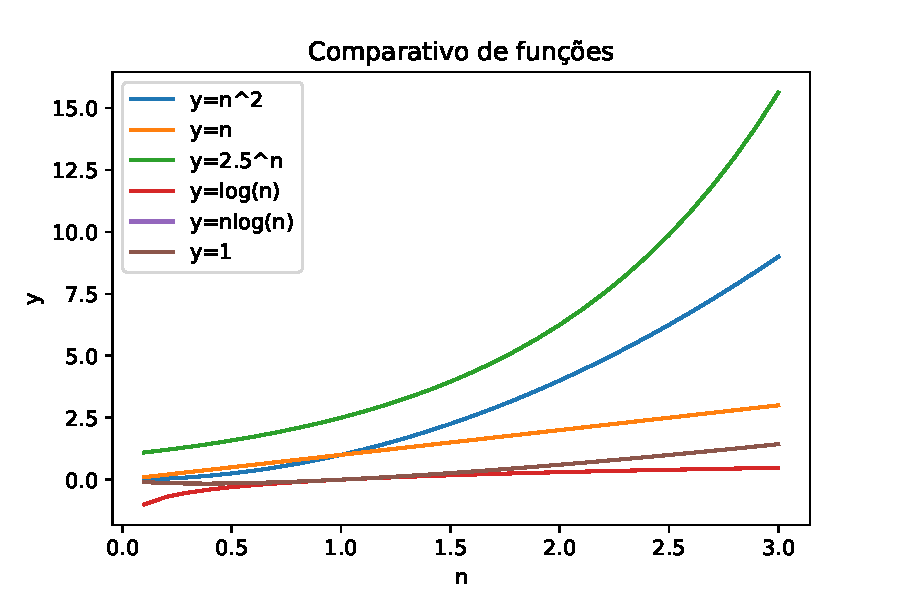
\includegraphics[scale=0.47]{./src/funcoes.pdf}\hspace{1cm}
\end{center}
}

\Sli{
No entanto, podemos generalizar a Equação 1 da seguinte forma:

\begin{equation}
\label{e.crescimento_assintotico_generalizado}
1 <\log(n)<\sqrt{n}<n<n\log(n)<n^2<n^3<\ldots<2^n<2.5^n<3^n<\ldots<n^n.
\end{equation}

\justify Qual a definição de $O(n)?$ 

\setbeamercolor{BoxColour}{fg=black,bg=gray!30}
\begin{beamercolorbox}[sep=1em,wd=13.4cm]{BoxColour}
   Uma função $f(n)\in O(g(n))$ sse $\exists c,n_o\in\mathbb{R}^+$ tal que $f(n)\leq cg(n)$, $\forall n\geq n_0$.
\end{beamercolorbox}\medskip

\justify \underline{Exemplo:} sejam as funções $f(n)=2n+3$ e $g(n)=n$. Assumindo que $c=10$ e $n_0=1$, temos que $f(n)\leq 10g(n)\implies2n+3\leq 10n$, $n\geq 1$. Assim sendo, temos que $f(n)\in O(g(n))$, ou seja, que $2n+3\in O(n)$. \textbf{Na prática, existem diversos valores para $c$ que satisfazem a relação $\bm{f(n)\in O(g(n))}$}.
}

\Sli{
\justify Vamos para um segundo exemplo. Continuemos assumindo que $f(n)=2n+3$, mas agora temos que $g(n)=n^2$. Pergunta: $f(n)\in O(g(n))$?

\justify Novamente, basta encontrarmos valores para $c$ e $n_0$ que satisfaçam a nossa definição anterior. Um exemplo seria $c=5$ e $n_0= 1$. Neste caso, teremos que $f(n)\leq 5g(n)\implies2n+3\leq5n^2$, $n \geq 1$. Novamente, temos que $f(n)\in O(g(n)$, ou seja, que $2n+3\in O(n^2)$. 

\justify Podemos continuar com outros exemplos e veremos que $2n+3\in O(n^3)$, e assim por diante. Assim, podemos estabelecer uma definição para \textbf{informal} para a notação $O$.

\begin{equation*}
1 <\log(n)<\sqrt{n}<\overbrace{n<n\log(n)<n^2<n^3<\ldots<2^n<2.5^n<3^n<\ldots<n^n}^{\in O(n)}.
\end{equation*}
}

\Sli{
\justify Agora vamos para a definição de limite inferior. \justify Qual a definição de $\Omega(n)?$

\setbeamercolor{BoxColour}{fg=black,bg=gray!30}
\begin{beamercolorbox}[sep=1em,wd=13.4cm]{BoxColour}
   Uma função $f(n)\in \Omega(g(n))$ sse $\exists c,n_o\in\mathbb{R}^+$ tal que $f(n)\geq cg(n)$, $\forall n\geq n_0$.
\end{beamercolorbox}\medskip

\justify \underline{Exemplo:} sejam as funções $f(n)=2n+3$ e $g(n)=n$. Assumindo que $c=1$ e $n_0=1$, temos que $f(n)\geq g(n)\implies2n+3\geq n$, $n\geq 1$. Assim sendo, temos que $f(n)\in \Omega(g(n))$, ou seja, que $2n+3\in O(n)$. \textbf{Note que também existem diversos valores para $c$ que satisfazem a relação $\bm{f(n)\in \Omega(g(n))}$}.

}

\Sli{
\justify Vamos para um segundo exemplo. Continuemos assumindo que $f(n)=2n+3$, mas agora temos que $g(n)=\log(n)$. Pergunta: $f(n)\in \Omega(g(n))$?

\justify Novamente, basta encontrarmos valores para $c$ e $n_0$ que satisfaçam a nossa definição de $\Omega(n)$. Um exemplo seria $c=1$ e $n_0=1$. Assim, teremos que $f(n)\geq g(n)\implies2n+3\geq\log(n)$, $n \geq 1$. Novamente, temos que $f(n)\in \Omega(g(n)$, ou seja, que $2n+3\in \Omega(\log(n))$. 

\begin{equation*}
\overbrace{1<\log(n)<\sqrt{n}<n}^{\in \Omega(n)}<n\log(n)<n^2<n^3<\ldots<2^n<2.5^n<3^n<\ldots<n^n.
\end{equation*}

}

\Sli{
\justify Agora vamos para a definição de limite médio. \justify Qual a definição de $\Theta(n)?$

\setbeamercolor{BoxColour}{fg=black,bg=gray!30}
\begin{beamercolorbox}[sep=1em,wd=14.4cm]{BoxColour}
   Uma função $f(n)\in \Theta(g(n))$ sse $\exists c_1,c_2,n_o\in\mathbb{R}^+$ tal que $c_1g(n)\leq f(n)\leq c_2g(n)$, $\forall n\geq n_0$.
\end{beamercolorbox}\medskip

\justify \underline{Exemplo:} sejam as funções $f(n)=2n+3$ e $g(n)=n$. Assumindo que $c_1=1$, $c_2=10$ e $n_0=1$, temos que $g(n)\leq f(n)\leq 10g(n)\implies n\leq2n+3\leq 10n$, $n\geq 1$. Assim sendo, temos que $f(n)\in \Theta(g(n))$, ou seja, que $2n+3\in \Theta(n)$. \textbf{Note que também existem diversos valores para $c_1$ e $c_2$ que satisfazem a relação $\bm{f(n)\in \Theta(g(n))}$}.
}

\Sli{
Desta forma, temos que:

\begin{equation*}
1<\log(n)<\sqrt{n}<\overbrace{n}^{\in \Theta(n)}<n\log(n)<n^2<n^3<\ldots<2^n<2.5^n<3^n<\ldots<n^n.
\end{equation*}

\justify Podemos, então, resumir o que aprendemos da seguinte forma: para uma função $f(n)=n$, temos que:

\setbeamercolor{BoxColour}{fg=black,bg=gray!30}
\begin{beamercolorbox}[sep=.1em,wd=14.4cm]
{BoxColour}
\begin{equation*}
\overunderbraces{&\br{2}{f(n) \in O(n)}&}%
{1<\log(n)<\sqrt{n}<&n&<n<\log(n)<n^2<n^3<\ldots<2^n<2.5^n<3^n<\ldots<n^n}
{\br{2}{f(n)\in\Omega(n)}&&}
\end{equation*}
\end{beamercolorbox}\medskip
Note que $n\in\Theta(n)$.
}

\SliT{Propriedades de Notações Assintóticas}{

\justify Propriedades gerais:

\begin{itemize}
	\item Se $f(n)\in O(g(n))$, então $af(n)\in O(g(n))$, $a\in\mathbb{R}$.\newline
	\underline{Exemplo:} seja $f(n)=2n^2+5\in O(n^2)$. Suponha $a=7$, então temos que $7f(n)=7(2n^2+5)=14n^2+35\in O(n^2)$.
	\item Se $f(n)\in \Omega(g(n))$, então $af(n)\in \Omega(g(n))$, $a\in\mathbb{R}$.\newline
	\underline{Exemplo:} seja $f(n)=2n^2+5\in \Omega(n^2)$. Suponha $a=7$, então temos que $7f(n)=7(2n^2+5)=14n^2+35\in \Omega(n)$.
\end{itemize}
A mesma propriedade também é válida para o simbolismo $\Theta(n)$.
}

\Sli{
\justify Propriedade \textbf{reflexiva}:

\begin{itemize}
	\item Dada $f(n)$, então $f(n)\in O(f(n))$.
	\item Dada $f(n)$, então $f(n)\in \Omega(f(n))$.
\end{itemize}

\justify Propriedade \textbf{transitiva}:
\begin{itemize}
	\item Se $f(n)\in O(g(n))$ e $g(n)\in O(h(n))$, então $f(n)\in O(h(n))$.\newline
	\underline{Exemplo:} sejam $f(n)=n$, $g(n)=n^2$ e $h(n)=n^3$. Temos que $n\in O(n^2)$ e $n^2\in O(n^3)$. É verdade, também, que $n\in O(n^3)$.
\end{itemize}
Esta propriedade também vale para os casos de $\Omega(n)$ e $\Theta(n)$.
}

\Sli{
\justify Propriedade \textbf{simétrica}:

\begin{itemize}
	\item Se $f(n)\in \Theta(g(n))$, então $g(n)\in \Theta(f(n))$. \textbf{Note que esta propriedade vale somente para a notação $\bm{\Theta}$}.\newline
	\underline{Exemplo:} sejam $f(n)=n^2$ e $g(n)=n^2$. Temos que $f(n)\in \Theta(n^2)$ e $g(n)\in\Theta(n^2)$. 
\end{itemize}

\justify Propriedade \textbf{simétrica transposta}:

\begin{itemize}
	\item Se $f(n)\in O(g(n))$, então $g(n)\in \Omega(f(n))$.\newline
	\underline{Exemplo:} sejam $f(n)=n$ e $g(n)=n^2$. Temos que $n\in O(n^2)$ e $n^2\in\Omega(n)$.
	\item Se $f(n)\in \Omega(g(n))$, então $g(n)\in O(f(n))$.\newline
	\underline{Exemplo:} sejam $f(n)=n^2$ e $g(n)=n$. Temos que $n^2\in \Omega(n)$ e $n\in O(n^2)$.
\end{itemize}
Caso $f(n)\in O(g(n))$ e $f(n)\in \Omega(g(n))$, então $f(n)\in \Theta(g(n))$.
}

\Sli{
\justify Caso $f(n)\in O(g(n))$ e $d(n)\in O(e(n))$, então $f(n)+d(n)\in O(\max(g(n),e(n)))$.\newline
	\underline{Exemplo:} sejam $f(n)=n\in O(n)$ e $g(n)=n^2\in O(n^2)$. Temos que $f(n)+d(n)=n+n^2$. Neste caso, temos que $n+n^2\in O(n^2)$.\newline
	
\centerline{
\setbeamercolor{BoxColour}{fg=black,bg=gray!30}
\begin{beamercolorbox}[sep=1em,wd=12.4cm]
{BoxColour}
Usualmente, a complexidade final é dada pelo polinômio de maior grau.
\end{beamercolorbox}\medskip
}

\justify Caso $f(n)\in O(g(n))$ e $d(n)\in O(e(n))$, então $f(n)d(n)\in O(g(n)e(n)))$.\newline
	\underline{Exemplo:} sejam $f(n)=n\in O(n)$ e $g(n)=n^2\in O(n^2)$. Temos que $f(n)d(n)=nn^2=n^3$. Neste caso, temos que $n^2\in O(n^3)$.
}

\SliT{Comparando Funções}{

\justify Dadas duas funções $f(n)$ e $g(n)$, como podemos compará-las, ou seja, quem cresce/decresce mais rapidamente?

\justify \underline{Exemplo:} sejam $f(n)=n^2$ e $g(n)=n^3$. Podemos \textbf{amostrar} alguns valores das funções e ver como eles se comportam. No caso abaixo, alguns poucos valores de $n$ são suficientes para dizer que $n^2<n^3$ para $n\rightarrow\infty$.

\begin{table}
\begin{tabular}{lcc}
  & \bm{$n^2$} & \bm{$n^3$}\\
$n=1$ & 1 & 1\\
$n=2$ & 4 & 8\\
$n=3$ & 9 &	27\\
\end{tabular}
\end{table}
}

\Sli{

\justify Uma outra abordagem para comparar funções corresponde à aplicação da \textbf{função} $\log$ em ambos lados, ou seja, $\log(n^2)$ e $\log(n^3)$. Temos que $\log(n^2)=2\log(n)$ e $\log(n^3)=3\log(n)$. Definitivamente, $2\log(n)<3\log(n)$. 

\justify Vejamos um outro exemplo de comparação de funções um pouco mais complexas, com as regras de logaritmos ao lado.

\begin{minipage}{0.697\textwidth}
\begin{table}
\begin{tabular}{lcc}
& $n^2\log(n)$ & $n(\log(n))^{10}$\\
 $\log\Rightarrow$ & $\log(n^2\log(n))$ & $\log(n(\log(n))^{10})$\\
 Regra 1 $\Rightarrow$& $\log(n^2)+\log(\log(n))$ & $\log(n)+\log(\log(n))^{10}$\\
 Regra 3 $\Rightarrow$ & $\underbrace{2\log(n)}_{\text{maior termo}}+\log(\log(n))$ & $\underbrace{\log(n)}_{\text{maior termo}}+10\log(\log(n))$\\
\end{tabular}
\end{table}
\end{minipage}%%% to prevent a space
\begin{minipage}{0.37\textwidth}
\begin{color}{blue}
\begin{color}{black}1.\end{color} $\log(ab) = \log(a)+\log(b)$\newline
\begin{color}{black}2.\end{color} $\log(a/b) = \log(a)-\log(b)$\newline
\begin{color}{black}3.\end{color} $\log(a^b) = b\log(a)$\newline
\begin{color}{black}4.\end{color} $a^{\log_c(b)} = b^{\log_c(a)}$\newline
\begin{color}{black}5.\end{color} $a^b=n\implies b=\log_a(n)$
\end{color}
\null
\par\xdef\tpd{\the\prevdepth}
\end{minipage}
Comparando apenas os maiores termos, temos que $n^2\log(n)>n(\log(n))^{10}$.
}

\Sli{

\justify Vejamos um outro exemplo. Agora temos que $f(n)=3n^{\sqrt{n}}$ e $g(n)=2^{\sqrt{n}\log(n)}$. Aqui, não iremos aplicar o $\log$, apenas as fórmulas de propriedade dos logaritmos.

\begin{minipage}{0.697\textwidth}
\begin{table}
\begin{tabular}{lcc}
& $3n^{\sqrt{n}}$ & $2^{\sqrt{n}\log(n)}$\\
 Regra 3 $\Rightarrow$ & $3n^{\sqrt{n}}$ & $2^{\log(n)^{\sqrt{n}}}$\\
 Regra 4 $\Rightarrow$& $3n^{\sqrt{n}}$ & $(n^{\sqrt{n}})^{\cancelto{1}{\log_2(2)}}$\\
 & $3n^{\sqrt{n}}$ & $n^{\sqrt{n}}$\\
\end{tabular}
\end{table}
\end{minipage}%%% to prevent a space
\begin{minipage}{0.37\textwidth}
\begin{color}{blue}
\begin{color}{black}1.\end{color} $\log(ab) = \log(a)+\log(b)$\newline
\begin{color}{black}2.\end{color} $\log(a/b) = \log(a)-\log(b)$\newline
\begin{color}{black}3.\end{color} $\log(a^b) = b\log(a)$\newline
\begin{color}{black}4.\end{color} $a^{\log_c(b)} = b^{\log_c(a)}$\newline
\begin{color}{black}5.\end{color} $a^b=n\implies b=\log_a(n)$
\end{color}
\null
\par\xdef\tpd{\the\prevdepth}
\end{minipage}
Como temos um fator multiplicador de $3$, podemos concluir que $3n^{\sqrt{n}}>n^{\sqrt{n}}$ (em termos de \textbf{quantidade}). Note que as funções são iguais \textbf{assintoticamente}.
}

\Sli{
\justify Vejamos um outro exemplo. Suponha as seguintes funções:

\begin{table}
\begin{tabular}{cc}
\begin{equation*}
	f(n) = \begin{cases}
                n^3 \text{ se $n<100$} \\
				n^2\text{ se $n\geq100$}
			\end{cases}
\end{equation*} &
\begin{equation*}
	g(n) = \begin{cases}
                n^2 \text{ se $n<10.000$} \\
				n^3\text{ se $n\geq10.000$}
			\end{cases}
\end{equation*}
\end{tabular}	
\end{table}

\begin{center}
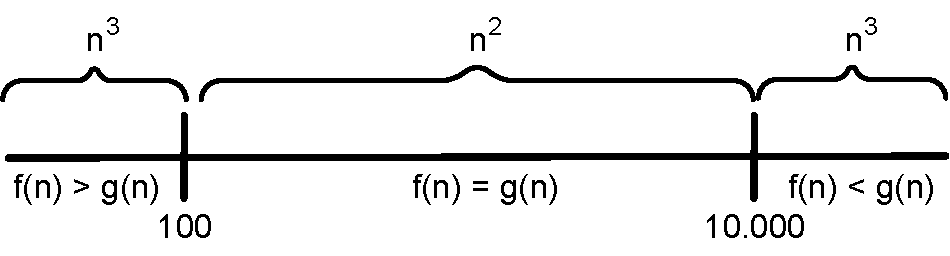
\includegraphics[scale=0.57]{./figs/rule.pdf}
\end{center}
Desta forma, podemos concluir que $g(n)>f(n)$ quando $n\rightarrow\infty$.
}

\Sli{

\justify Verdadeiro ou falso?

\begin{enumerate}
	\item $(n+k)^m\in \Theta(n^m)$?
	\item $2^{n+1}\in O(2^n)$?
	\item $2^{2n}\in O(2^{2n})$?
	\item $\sqrt{\log(n)}\in O(\log(\log(n)))$?
	\item $n^{\log(n)}\in O(2^n)$?
\end{enumerate}
}

\SliT{Considerações finais}{

\begin{itemize}
	\item Crescimento assintótico de funções estuda o comportamento delas em função do tempo e do tamanho da entrada $n$.
	\item Notações mais importantes: $\Theta$ e $O$.
	\item Funções podem ser assintoticamente similares mas com quantidades diferentes. 
	\item Em funções polinomiais, a complexidade final é dada pelo polinômio de maior grau.
\end{itemize}
}

\end{document}